La realización de este proyecto ha permitido alcanzar los objetivos que se planteaban al comienzo del mismo. En primer lugar se han investigado y evaluado diferentes formas y algoritmos para abordar la problemática inicial. Como consecuencia de ello se seleccionó la aproximación de Ellis al Vocoder de Fase. Posteriormente, trabajar en la implementación del prototipo ha permitido generar una versión parcialmente funcional del mismo en la placa proporcionada, en la que se han estudiado diferentes formas de lidiar con la problemática derivada del diseño, siendo necesario añadir modificaciones en el mismo a lo largo del periodo de trabajo. 

Es evidente que todo ello ha significado la consecución del objetivo último consistente en sintetizar y afianzar los conocimientos utilizados dentro de los diferentes ámbitos del proyecto: teoría de la señal y procesado de la misma, programación hardware y lenguaje VHDL, ciclo de desarrollo de un producto y finalmente electrónica analógica de adecuación de señal.

\begin{figure}[!b]
\begin{center}
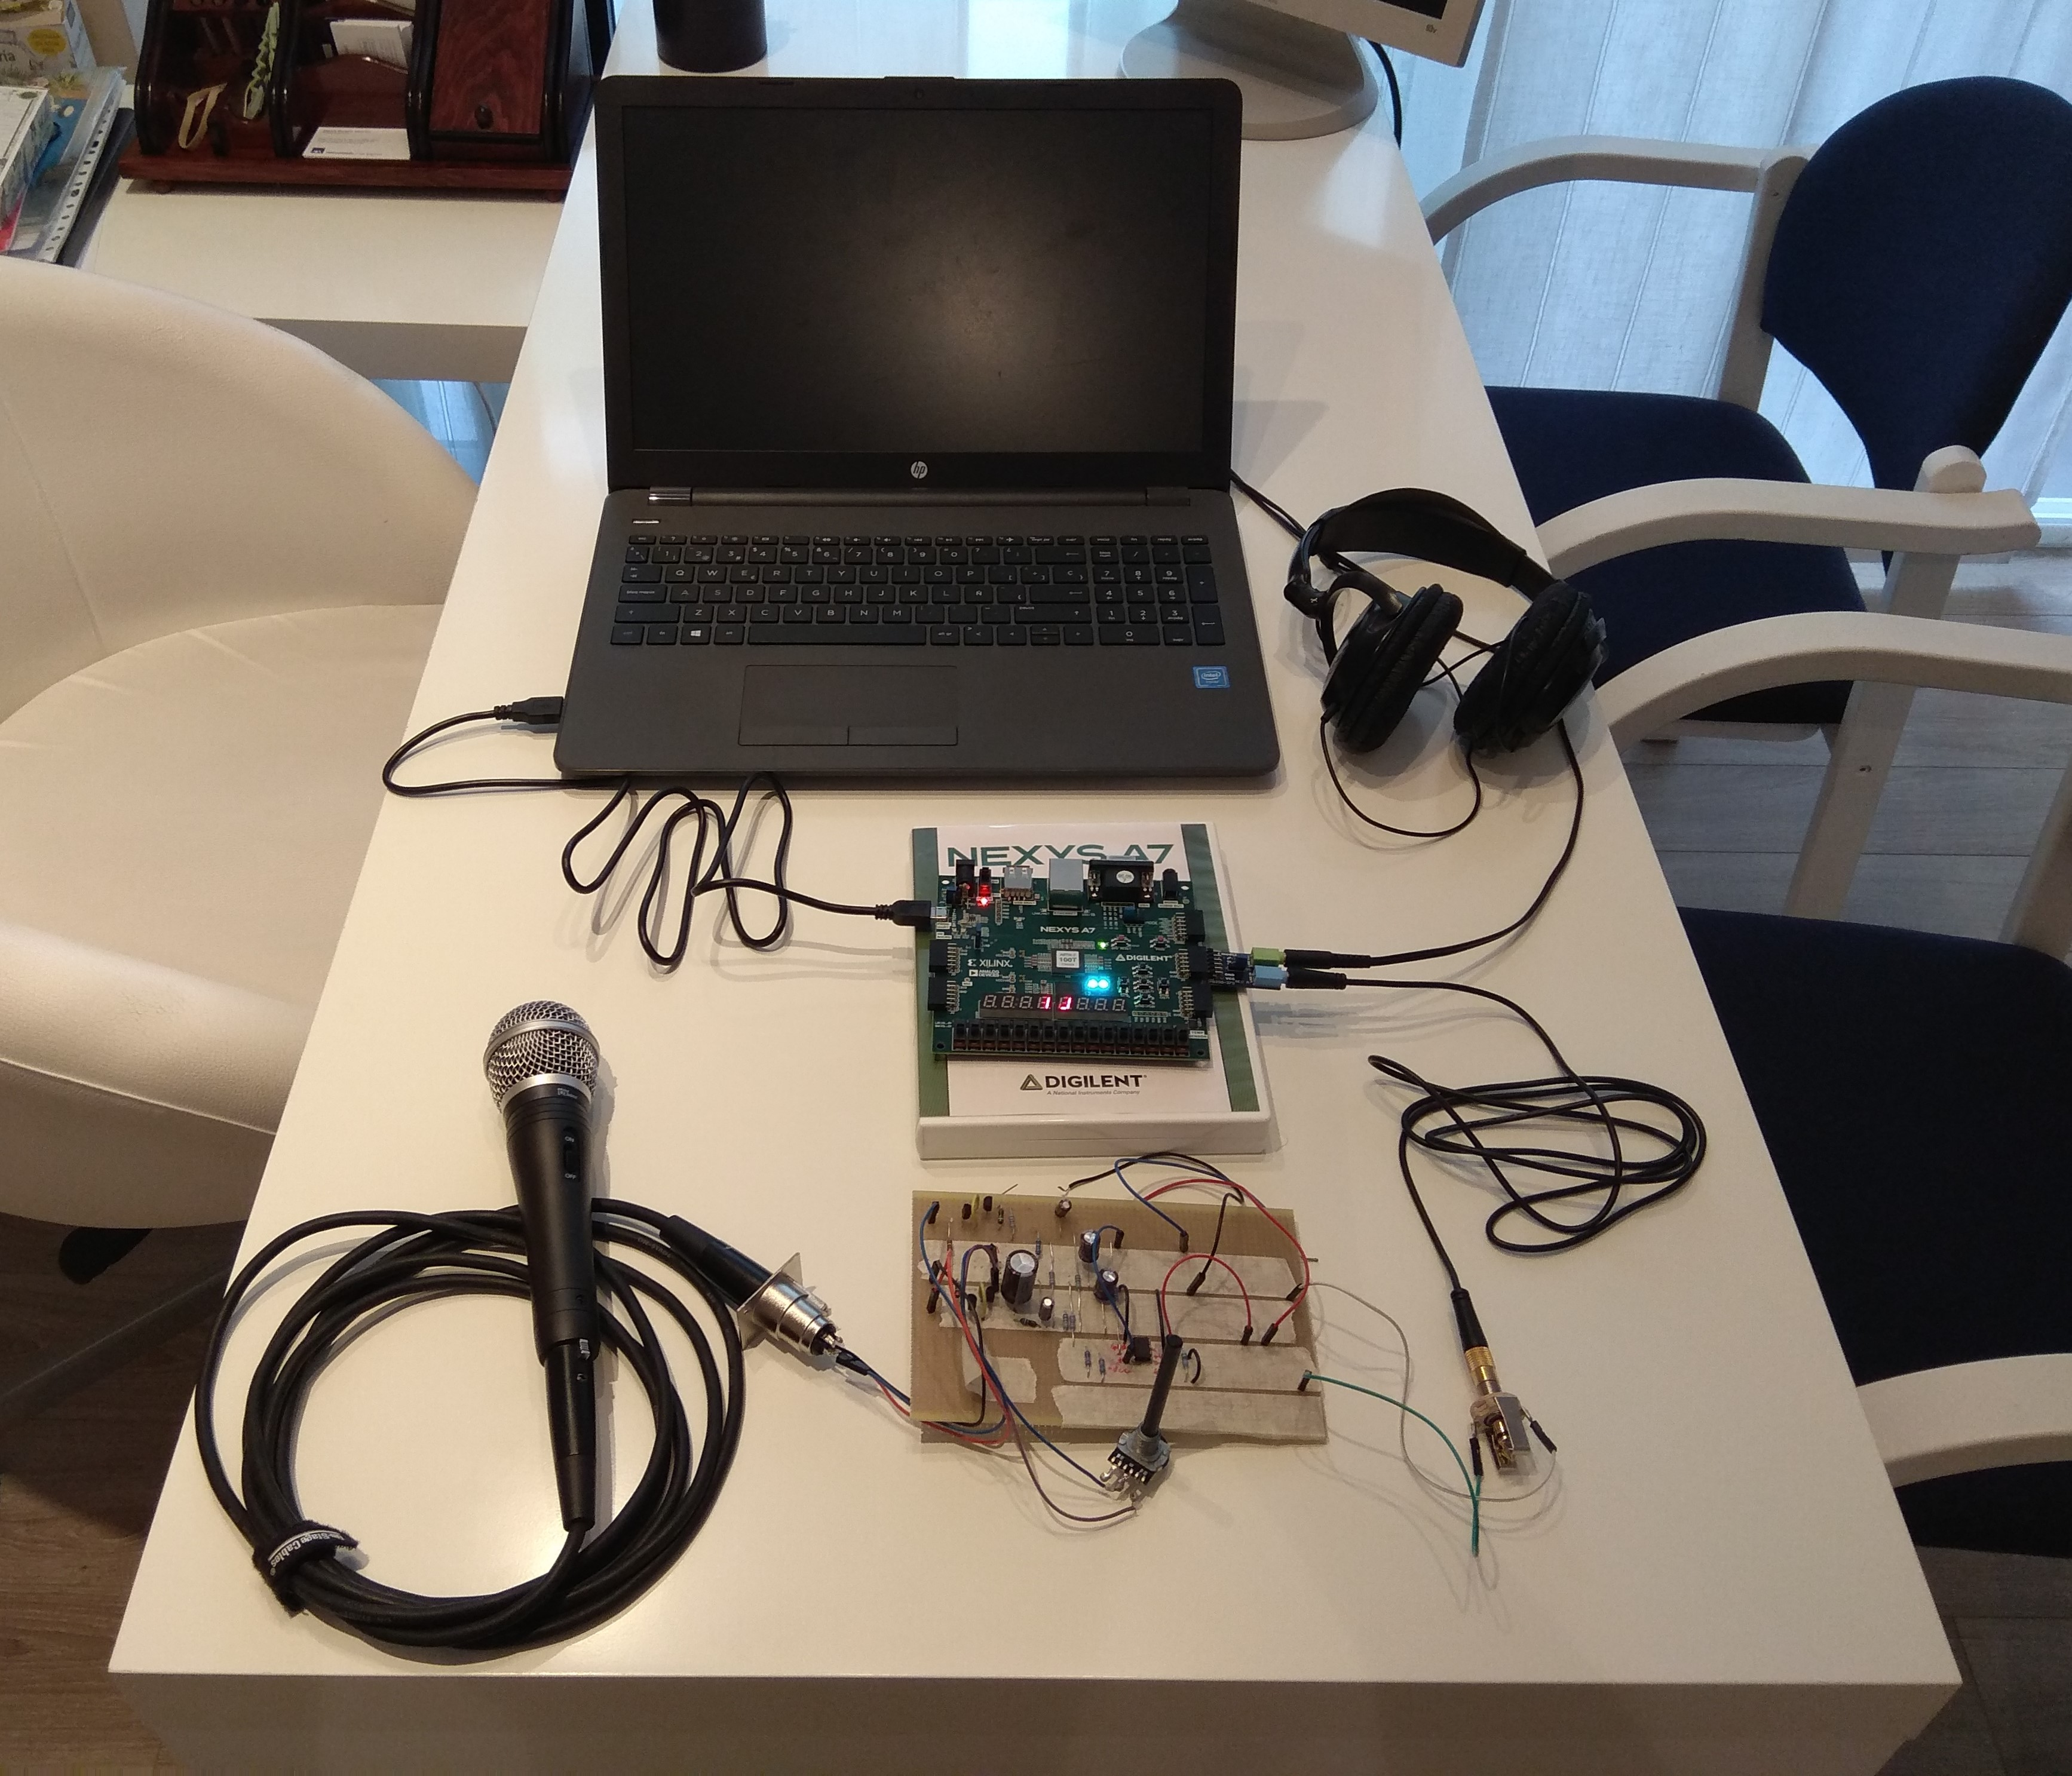
\includegraphics[width=10cm]{img/final.jpg}
%\caption{\label{fig:final}Conjunto final de los módulos desarrollados}
\end{center}
\end{figure}

Sin embargo, no ha sido posible completar la implementación del prototipo en el tiempo disponible, debido a que el ciclo de desarrollo de un aparato de estas características supera con creces la longitud del curso académico. Teniendo en cuenta la enorme cantidad de dificultades que han ido surgiendo a lo largo de este tiempo debido a lo novedoso del tema para mí y la dificultad para encontrar literatura útil para solucionarlos, me considero más que satisfecho con los resultados obtenidos.

De cara a futuras ampliaciones sobre el tema, sería interesante culminar la realización del prototipo para permitir realmente medir su latencia real y su calidad en el procesado. Una vez obtenidos estos datos, se podría mejorar el diseño optimizando las etapas existentes en el mismo, como usando módulos FFT específicos, experimentando con diferentes longitudes de palabra, de las ventanas y de las transformadas, tomando medidas en todos estos casos. Una vez realizadas se podría establecer una comparación útil con otras propuestas ya existentes para evaluar las fortalezas y debilidades de la implementación realizada. 

